\chapter{The \glsentrylong{lartpc}}
\label{chap:lartpc}

\glsreset{lar}
\glsreset{tpc}

The \gls{tpc} is a derivative of Charpak's \gls{mwpc}~\cite{mwpc}, developed by Nygren in the late 1970s~\cite{nygrenTPC}.
Crossing charged particles ionise the detection medium, which was gaseous in the original design.
An electric field is applied to prevent the recombination of the ions and electrons.
In this field the electrons drift towards a \gls{2d} readout plane (an \gls{mwpc} in the original design).
The charge readout is triggered by a scintillation light readout, also providing accurate timing of an event.
This allows to measure the time for the ionisation electrons to reach the readout plane.
As the drift speed of charged particles in the detection medium is constant and provided it is known, the coordinate in drift direction can be calculated from the drift time.

While gaseous \glspl{tpc} already provide very accurate tracking, they have the disadvantage that the target mass and thus the cross-section of the detection medium is quite low, resulting in a low interaction rate.
In 1977 Rubbia proposed the usage of \lar{} as a detection medium to solve this problem~\cite{lartpc}.
This requires a cryogenic detector while gaseous detectors can be operated at room temperature.
The type of \lartpc{} investigated in this work is fully emerged in \lar{} and is called single-phase.
A slightly altered scheme uses avalanche charge amplification to improve the \gls{snr}.
As of today, avalanche amplification is only possible with the charge readout situated in a gas phase above the \lar{}.
The details of such a dual-phase design are out of the scope of this work, they have been described by Aprile et al.~\cite{NobleGasDetectors} for instance.


\section{\glsentrylong{lar} as a Detection Medium}
\label{sec:lartpc_lar}

For an efficient particle detection by a \gls{tpc} several properties of the sensitive medium are of interest, such as ionisation and light yield, electron-ion pair recombination, dielectric strength, length scales of \gls{em} and hadronic interactions, density, transparency to its own scintillation light, and the boiling point.
\lar{} is quite unique as it has all the necessary properties while at the same time it is comparably cheap because it is readily available in the Earth's atmosphere.
A summary of its properties can be found in Table~\ref{tab:lartpc_larprop}.
Xenon, for instance, slightly surpasses argon in many aspects but is prohibitively expensive to build large detectors.
A boiling point of $\approx \SI{87}{\kelvin}$ raises the need for strong thermal insulation and a potent cooling system for \lar{}, though the requirements are far less stringent then for liquid helium.
This section outlines the most important \lar{} properties.

\begin{table}[tbp]
	\centering
	\caption[\glsentryshort{lar} properties]{%
		Properties of \acrshort{lar}, taken from~\cite{NobleGasDetectors} where not specified otherwise.
		}
	\label{tab:lartpc_larprop}
	\begin{tabu} to \textwidth {llSs}
		\toprule
		Property &									Symbol &				{Value} &	{Unit} \\
		\midrule
		Molar mass &								$\mu$ &					3.9948e1 &	\gram\per\mol \\
		Boiling point at \SI{1.01325e5}{\pascal} &	$T_{\m{S}}$ &			8.726e1 &	\kelvin \\
		Density at $T_{\m{S}}$ &					$\rho_{\m{S}}$ &		1.399e3 &	\kilo\gram\per\cubic\metre \\
		Dielectric constant~\cite{dielConst} &		$\varepsilon_{\m{r}}$ &	1.504 &		\\
		Required energy per electron-ion pair &		$W_{\m{i}}$ &			2.36e1 &	\electronvolt \\
		Required energy per photon &				$W_{\m{sc}}$ &			1.95e1 &	\electronvolt \\
		Fano factor &								$F$ &					1.07e-1 &	\\
		\acrshort{em} radiation length &			$X_{\m{0}}$ &			1.4e-1 &	\metre \\
		Hadronic interaction length &				$\lambda_{\m{int}}$ &	8.37e-1 &	\metre \\
		Peak scintillation wavelength &				$\lambda_{\m{scint}}$ &	1.28e-7 &	\metre \\
		Scintillation attenuation length &			$\lambda_{\m{att}}$ &	6.6e-1 &	\metre \\
		Concentration in air by volume &			&						9.34e-1 &	\percent \\
		\bottomrule
	\end{tabu}
\end{table}

Two processes are crucial to the registration of ionisation tracks of charged particles in a \gls{tpc}: charge production and transport.
The charge production needs to be high enough to be detectable by the available electronics.
This is given by the energy required to produce an electron-ion pair $W_{\m{i}}$.
The $W_{\m{i}}$ value of \SI{23.6}{\electronvolt} for \lar{} is challenging but manageable with contemporary electronics, as will be shown in Section~\ref{sec:lartpc_electronics}.
Naturally, this imposes a lower limit on detectable $\frac{\m{d}E}{\m{d}x}$.

Free electron transport is mainly influenced by three processes: \emph{recombination}, \emph{diffusion}, and \emph{lifetime}.
The ultimate goal is to collect as much of the produced charge as possible.
Recombination is the main process opposing this.
While it can be partially mitigated by increasing the electric field, it cannot be eliminated completely.
Even if that was possible, it would not be beneficial because the scintillation light needed for the drift time measurement is partly produced by recombining electron-ion pairs.
The relation between drift field strength and charge yield can be described by the \emph{box model}~\cite{box-model}.
It assumes that the ion-electron pairs are isolated and initially uniformly populate a box of a given size.
Furthermore, the diffusion of electrons and ions as well as the ion drift velocity (\num{1e5} times smaller than for electrons) are assumed to be negligible.
For a produced charge $Q_{\m{0}}$ and a collected charge $Q$ the collection ratio is given by
\begin{IEEEeqnarray}{rCl}
	\frac{Q}{Q_{\m{0}}} & = & \frac{1}{\xi} \ln(1 + \xi)
	\label{eq:lartpc_lar-reco}
\end{IEEEeqnarray}
with a parameter $\xi$ depending on the drift field, electron mobility, initial number of electron-ion pairs, chosen size of the box and recombination coefficient.
Figure~\ref{fig:lartpc_box-model} shows a measurement by \gls{help} of the collected charge in an \SI{8}{\milli\metre}-drift \lartpc{} for various drift field intensities and concentrations of nitrogen mixed into the \lar{}.

\begin{figure}[tbp]
	\centering
	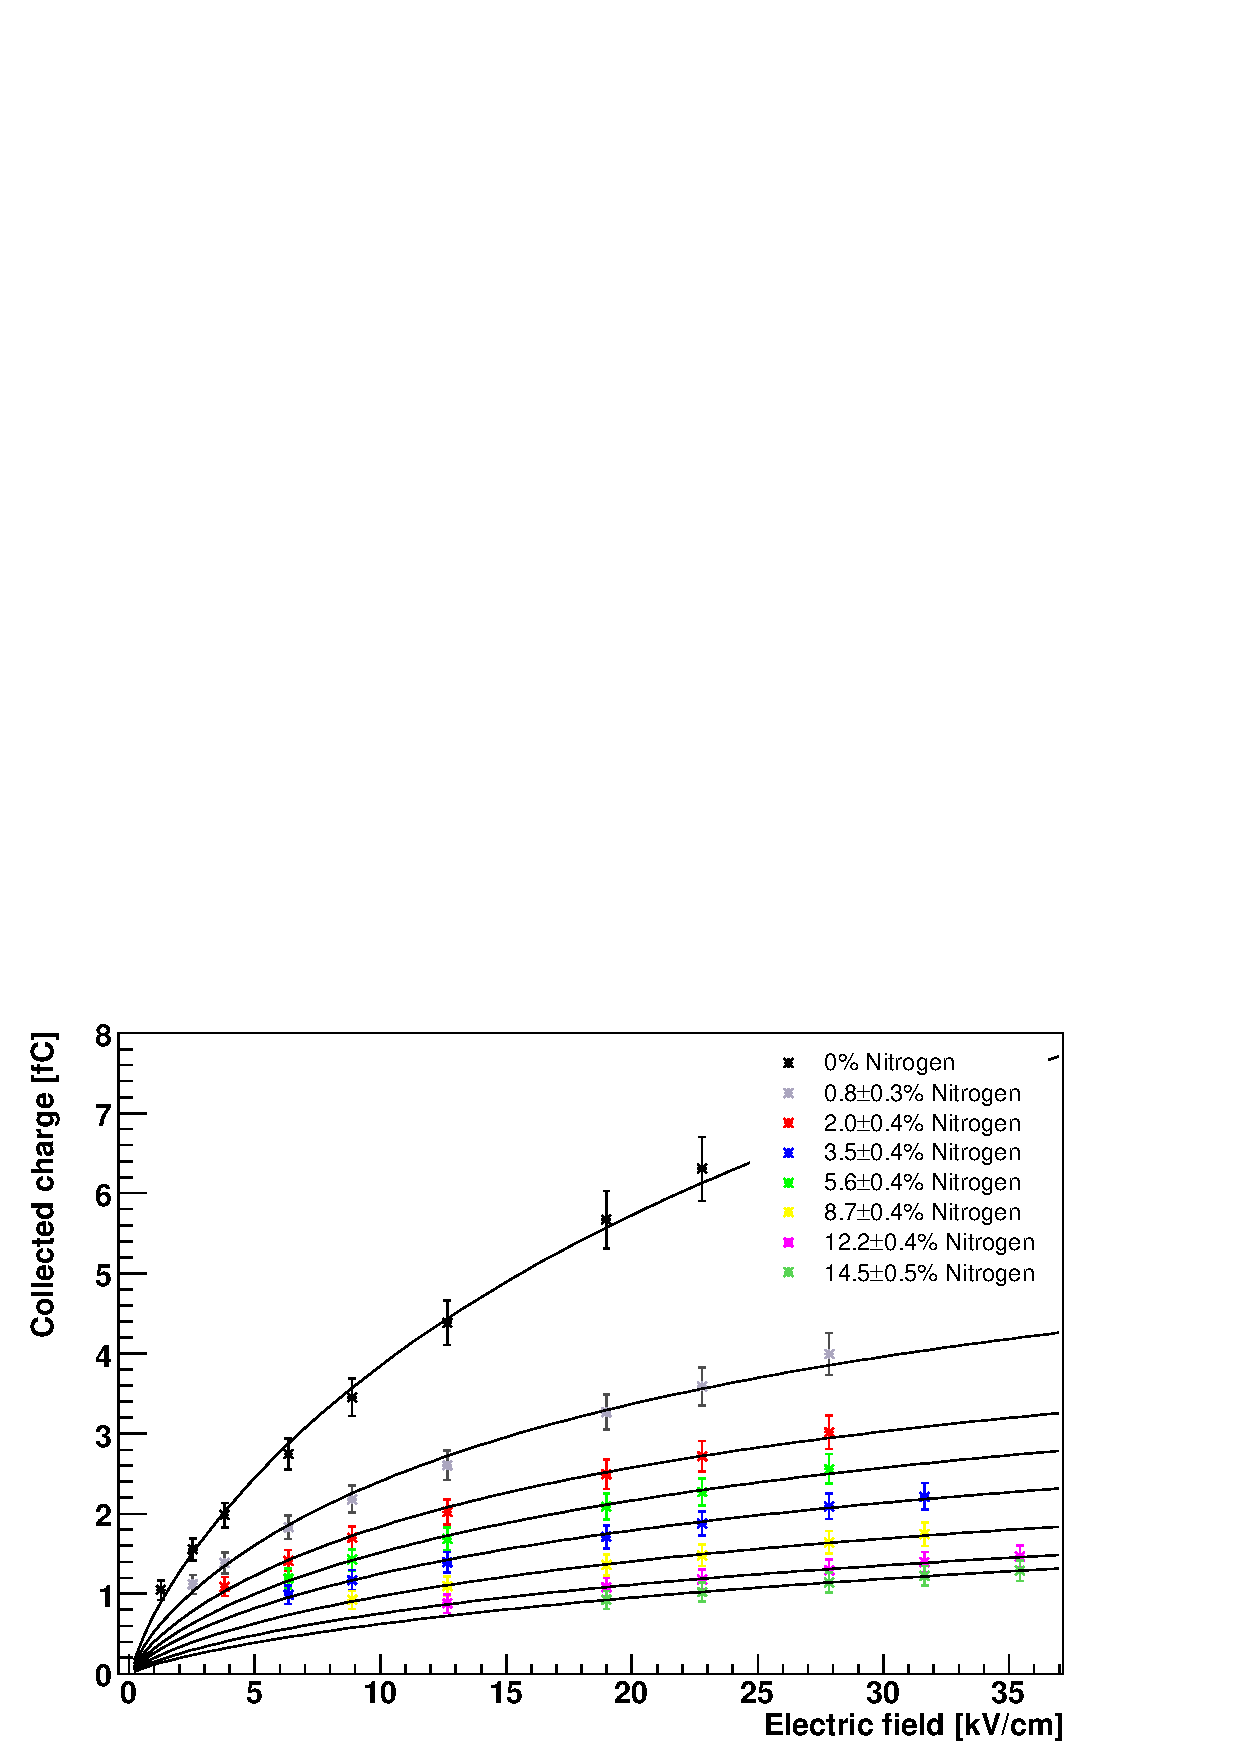
\includegraphics[viewport=14 5 511 351, clip, width=\textwidth]{lartpc/box-model}
	\caption[\glsentryshort{lar} recombination measurements]{%
		Collected charge in an \SI{8}{\milli\metre}-drift \acrshort{lartpc} as a function of electric field, for various concentrations of nitrogen mixed into the \acrshort{lar}.
		The lines represent box model fits.~\cite{grna-lhep}
	}
	\label{fig:lartpc_box-model}
\end{figure}

Ionisation charge clouds will start to diffuse over time due to thermal motion.
The process is characterised by the diffusion coefficient $D$.
In the presence of a drift field longitudinal ($D_{\m{L}}$) and transversal ($D_{\m{T}}$) components need to be treated separately.
The resulting smearing of the ionisation charge cloud after a drift time $t$ is given by
\begin{IEEEeqnarray}{rCl}
	\sigma_{\m{L/T}} & = & \sqrt{2 D_{\m{L/T}} t}
	\label{eq:lartpc_lar-diff}
\end{IEEEeqnarray}
for longitudinal and transversal diffusion, respectively.
Therefore, $D$ has the dimension of area per time.~\cite{lngDet}

A third process affecting charge transport is electron trapping by impurities, the probability of an electron becoming attached to an atom in the medium.
For the argon itself this is highly unlikely because its outer electron shell is fully populated.
This is one of the reasons why (liquefied) noble gases are a prime choice for \glspl{tpc}.
Nevertheless, drifting electrons can be captured by impurities in the argon.
Oxygen is particularly bad due to its high electronegativity.
Impurities are therefore often measured in oxygen-equivalent concentration.
Finite purity gives rise to a finite lifetime of free electrons in the medium.
\begin{IEEEeqnarray}{rCl}
	N_{\Pe} \qty(t) & = & N_{\Pe} \qty(0) e ^ {- \frac{t}{\tau}}
	\label{eq:lartpc_lar-lifetime}
\end{IEEEeqnarray}
is the charge left after a time $t$ for an electron lifetime $\tau$.

The velocity of the charge drifting in an electric field is related to the mobility $\mu$ by
\begin{IEEEeqnarray}{rCl}
	\va{v} & = & \mu\qty(\va{E}) \va{E} \qc
\end{IEEEeqnarray}
where $\mu$ in general depends on the electric field and is different for electrons and ions.
This means that the higher the field is, the higher is the charge velocity and thus the lower the drift time.
Drift times need to be kept low for multiple reasons.
One of them are the aforementioned impurities.
A low lifetime caused by a high impurity concentration can be partially compensated by a higher field.
Increasing the drift time in an experiment exposed to high rates of cosmic radiation will increase pile-up, i.e.\ the number of events simultaneously present in the detector.
Pile-up in turn complicates event reconstruction.
On the other hand, the readout electronics need to be fast enough to guarantee the required spatial resolution in the drift coordinate, defining an upper limit for the drift velocity.
A reasonable value from a purity point of view is a drift time of $\sim{\SI{1}{\milli\second}}$.
For a detector size of $\sim{\SI{1}{\metre}}$ the required drift speed is $\sim{\SI{1}{\milli\metre\per\micro\second}}$, requiring a field of $\sim{\SI{1}{\kilo\volt\per\centi\metre}}$.

A drift field of \SI{1}{\kilo\volt\per\centi\metre} becomes challenging in detectors much larger than \SI{1}{\metre} due to the high required cathode voltage.
Soon after entering \lartpc{} R\&D, the \gls{help} group realised that the reported dielectric strength of \lar{} is much lower~\cite{breakdown_14} than measured by Swan et al.\ in 1960~\cite{swan1, swan2}.
It turned out, opposing the assumption of Swan et al., that the dielectric strength is not independent of the absolute dimensions of the electrodes.
This led to a very detailed study of breakdowns in \lar{} in the course of this thesis, which will be presented in Section~\ref{sec:studies_breakdown}.


\section{Electric Field Generation}
\label{sec:lartpc_efield}

\begin{figure}[tbp]
	\centering
	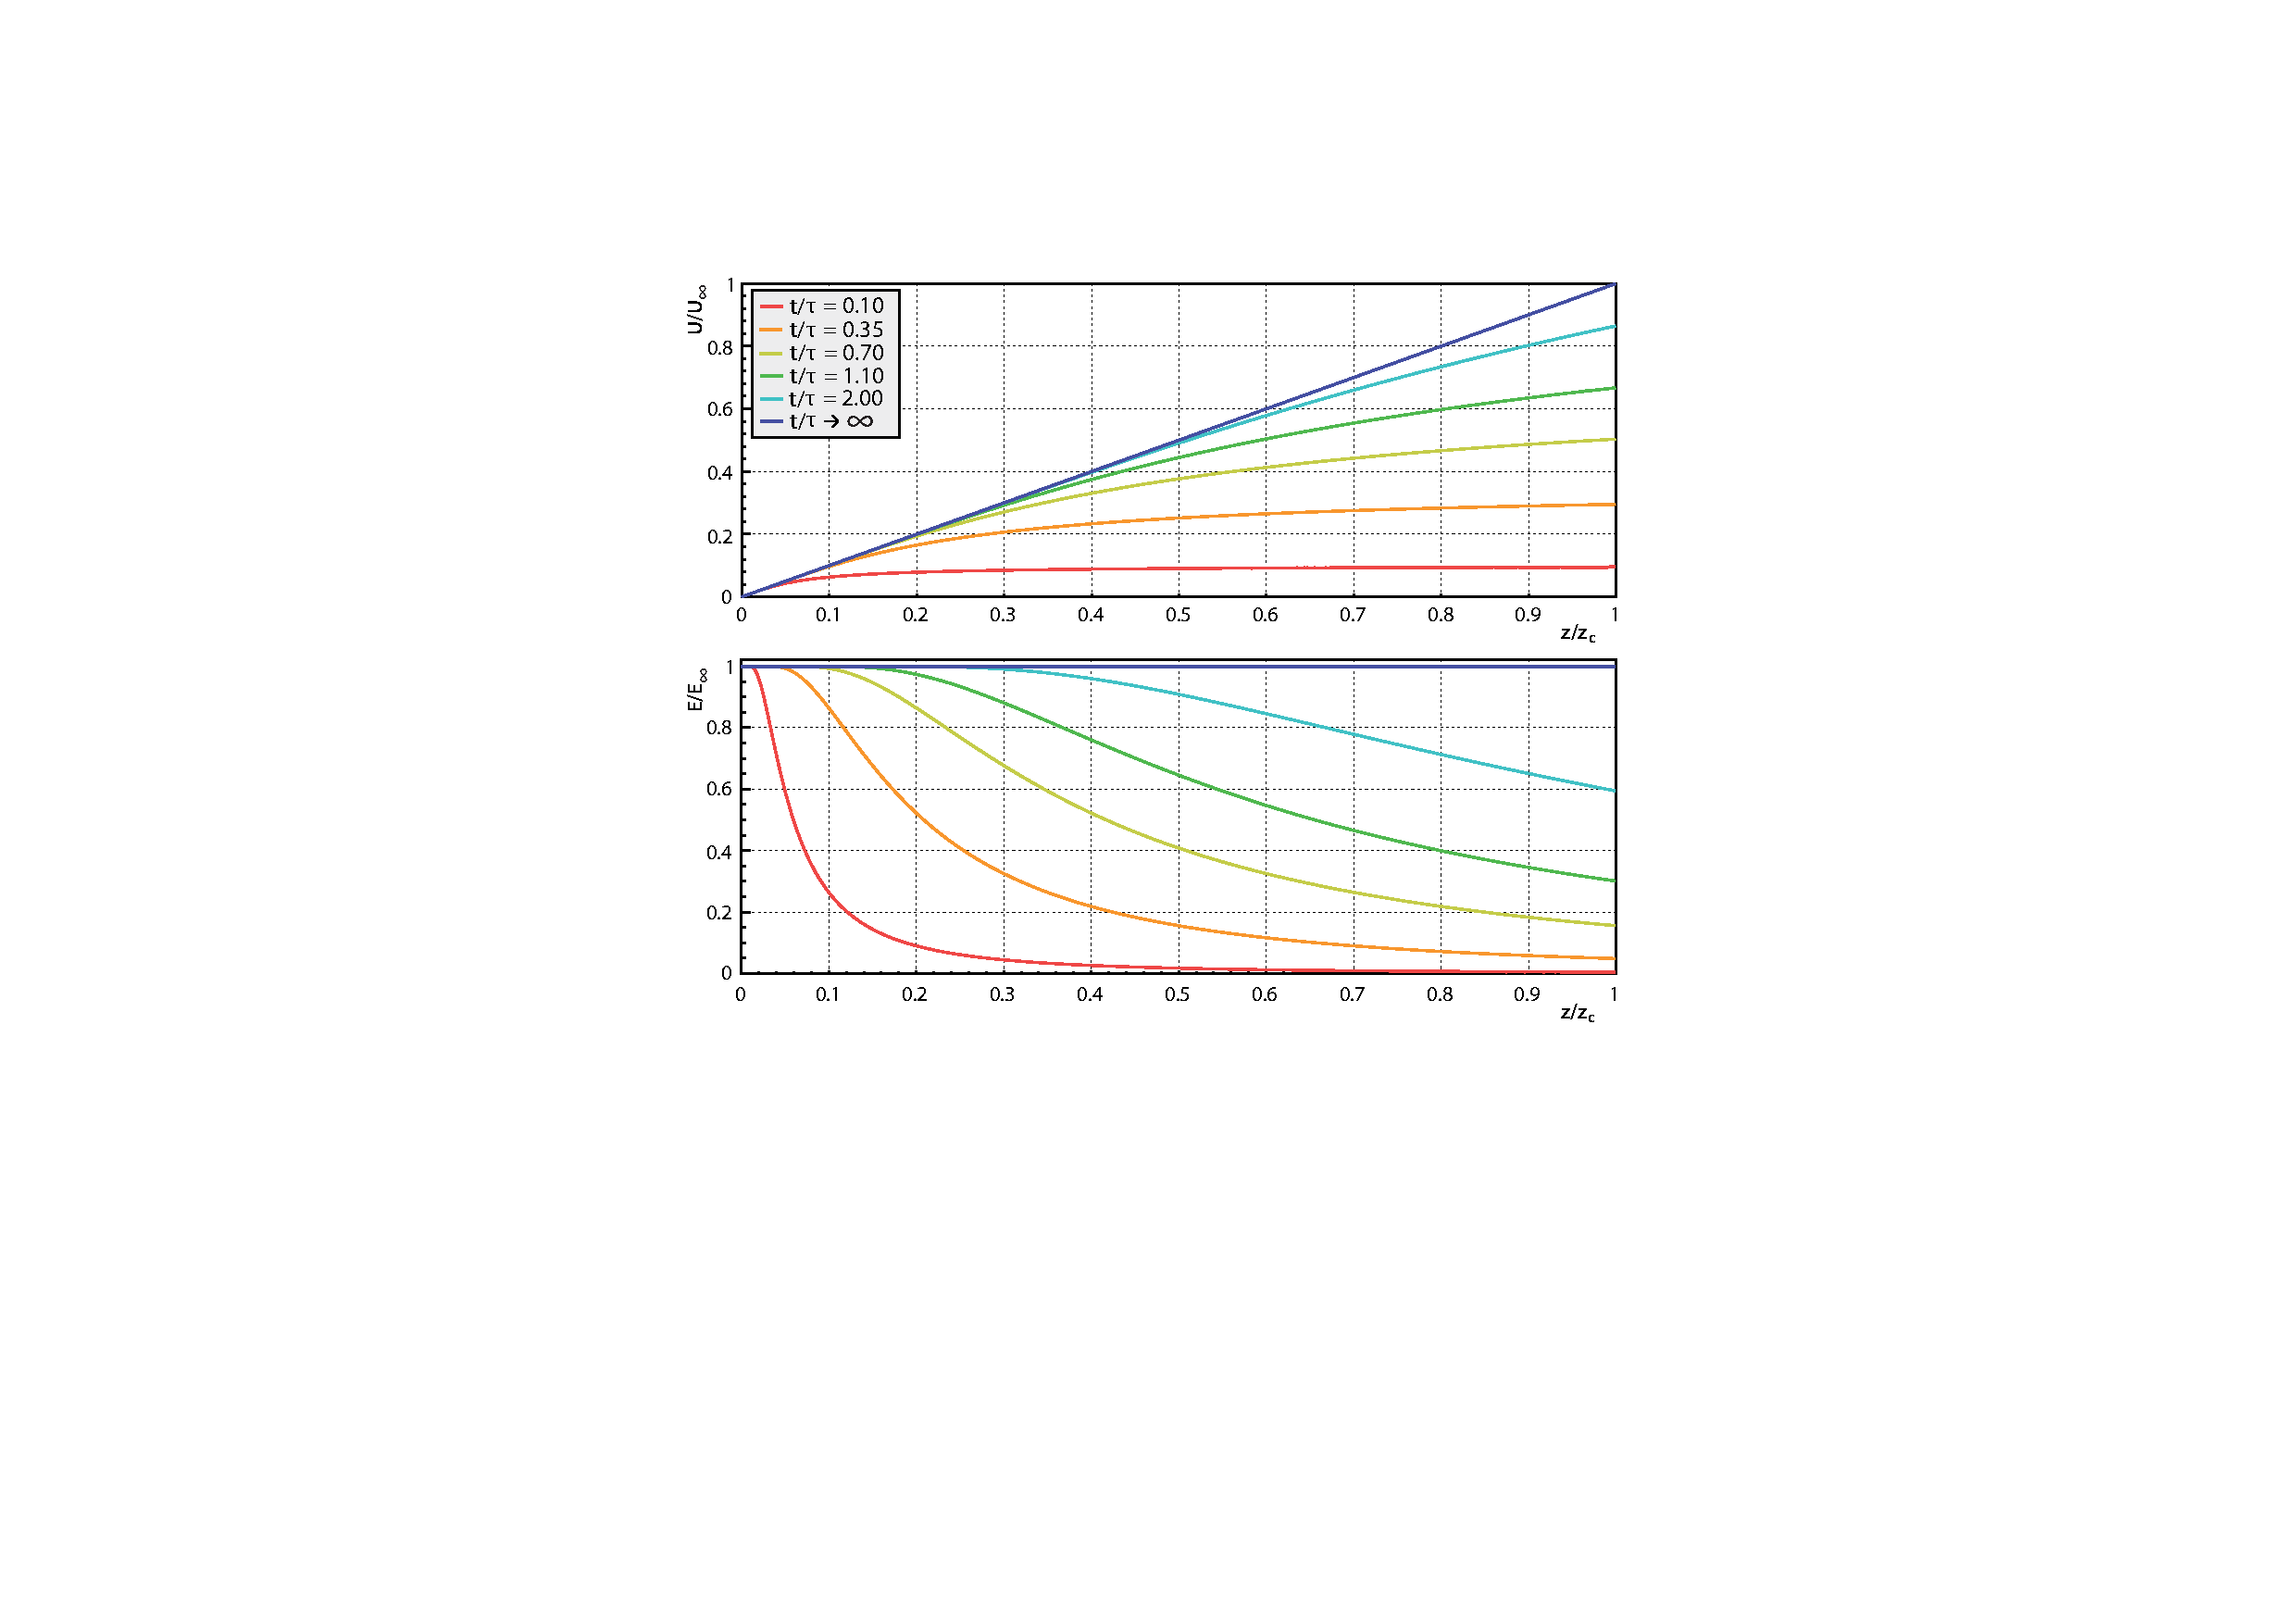
\includegraphics[width=\textwidth]{lartpc/greinacher}
	\caption[Voltage and electric field produced by a Greinacher voltage multiplier]{%
		Relative voltage ($U/U_{\infty}$, top) and longitudinal electric field ($E/E_{\infty}$, bottom) obtained with a Greinacher multiplier as a function of relative drift coordinate $z/z_{\m{c}}$, for different charging states $t/\tau$.
		The dark blue curves correspond to a fully charged Greinacher circuit.~\cite{AT_field}
	}
	\label{fig:lartpc_greinacher}
\end{figure}

For charge separation and drift an electric field of $\sim{\SI{1}{\kilo\volt\per\centi\metre}}$ is needed inside the fiducial volume of a \lartpc{}.
An easy way to achieve this is by means of field shaping rings fed by a resistive divider between cathode and anode.
The drawback is the need for a feedthrough capable of withstanding the full cathode voltage.
An alternative is to generate the \gls{hv} inside the cryostat, for instance using a Greinacher voltage multiplier circuit as the one used for the \AT{} experiment at \gls{help}~\cite{AT}.
A Greinacher multiplier works by pumping up a cascade of capacitors and diodes using a \gls{hf} source.
While the voltage generation worked well, this approach proved to be impractical because the \gls{hf} charging voltage interfered with the charge readout and therefore had to be turned off during data-taking.
Charging a Greinacher circuit is an asymptotic process, as can be seen in Figure~\ref{fig:lartpc_greinacher}.
It depicts voltage and resulting electric field as a function of drift distance for various charging states.
The characteristic charging time $\tau$ of \AT{} was $\sim \SI{10}{\minute}$.
Due to leakage currents and protection resistors the circuit needed frequent recharging: approximately \SI{1}{\minute} every \SI{15}{\minute}.
This caused a lot of detector down time, making a Greinacher circuit impractical for physics experiments.
More information on the \AT{} Greinacher multiplier can be found in~\cite{AT_field, maercu, michu}.


\section{Charge Readout}
\label{sec:lartpc_charge-ro}

Classically, the charge readout of a \lartpc{} is done using wires with a diameter of $\sim{\SI{.1}{\milli\metre}}$.
One wire plane delivers a \gls{2d} projection of the ionisation tracks in the detection medium.
This has two consequences:
\begin{enumerate}
	\item At least two parallel wire planes are needed to be able to reconstruct the \gls{3d} event topology.
	\item In theory, the more complex the event topology, the more planes are required to fully reconstruct it.
\end{enumerate}
Multiple wire planes can be realised by operating only the last one (in drift direction) in charge collection mode.
All the preceding wire planes are biased in such a way that they are transparent to the incoming charge but pick up an induction signal during the passage of the latter.
A typical number of wire planes for currently operational detectors is three, tilted at \ang{60} w.r.t.\ each other.


\section{Light Readout}
\label{sec:lartpc_light-ro}

Drift time needs to be measured to calculate the distance the charge has drifted along the electric field (i.e.\ the space coordinate perpendicular to the readout plane).
The \gls{daq} can record the time of the arrival of the charge at the readout plane.
What is missing is the time of charge production.
It can be acquired by registering the scintillation light produced alongside the ionisation of the detection medium.
Contemporary detector designs employ \glspl{pmt} for this purpose.
\glspl{pmt} are a well-established technology with a high quantum efficiency and fast response, but they require a lot of space.

A photon impinging on a \gls{pmt} is converted to an electron by a photocathode covering the sensitive surface of the \gls{pmt}.
These photo cathodes have a limited absorption spectrum.
In particular, the scintillation light of \lar{} does not fall inside the spectra of most photocathodes.
That is why the \gls{vuv} scintillation light needs to be converted to the visible range, where it can be efficiently detected by a \gls{pmt}.
\gls{tpb} is a widespread \gls{wls} capable of achieving this.
A common setup consists of coating either the \gls{pmt}~\cite{icarus} or a surface in front of it~\cite{uboone} with \gls{tpb}.


\section{Charge Readout Electronics}
\label{sec:lartpc_electronics}

This section gives an overview of charge readout electronics from the physics perspective.
A more detailed review will be given in Section~\ref{sec:studies_electronics}.
Using $W_{\m{i}}$, the energy required to produce one electron-ion pair, from Section~\ref{sec:lartpc_lar} and assuming a \gls{mip} in \lar{} (see Section~\ref{sec:nu-detection_fs}) one gets

\begin{IEEEeqnarray*}{rCl}
	\dv{Q}{x}	= \frac{\eval{\dv{E}{x}}_{\m{\glsentryshort{mip}}}}{W_{\m{i}}} \si{\elementarycharge}
			&	= & \frac{\SI{210}{\kilo\electronvolt\per\milli\metre}}{\SI{23.6}{\electronvolt}} \si{\elementarycharge}
				\approx \SI{8900}{\elementarycharge\per\milli\metre}
				\approx \SI{1.4}{\femto\coulomb\per\milli\metre}
\end{IEEEeqnarray*}

as a rough estimation for the charge yield.
This calculation does not incorporate recombination, diffusion, and charge lifetime, meaning that in a real experiment the value will be even lower.
The result is that the readout electronics need to be capable of detecting $\sim{\SI{1}{\femto\coulomb}}$ charges.

That is why the charge signal needs to be amplified before digitisation.
This is achieved by means of an integrating amplifier, converting the charge to a voltage.
Early \lartpc{} designs used preamplifiers outside the cryostat at room temperature.
From a noise point of view though it is beneficial to put the amplifiers inside the cryostat submerged in \lar{} for two reasons.
First, the closer to the source the amplifier is located, the shorter the low-signal lines will be, resulting in less pick-up noise.
Second, the temperature-dependent Johnson-Nyquist noise of the amplifiers will be reduced at cryogenic temperatures (see Section~\ref{sec:studies_electronics}).

For the same reasons it makes sense to operate the entire analogue signal chain at cryogenic temperatures.
This would also help to eliminate ground loops, which can pick up noise inductively or provoke self-oscillation of the analogue signal circuitry.
However, it is not easy to operate electronics at cryogenic temperatures.
Usually, a complete redesign of the circuit is necessary due to most components operating outside their guaranteed temperature range.
For some complex active components like the amplifiers and digitisers even a redesign of the \gls{ic} might be necessary.
On the other hand, placing the digitisers too close to the readout might result in elevated noise levels due to the digital clocks coupling into the analogue signal path.

The requirements on the electronics are given by the required sensitivity of the detector.
The necessary bit depth of the digitisers is given by the required dynamic range, i.e.\ the minimum and maximum amount of charge the readout needs to be able to register.
While the spatial resolution in the two coordinates parallel to the readout plane is given by the pitch of the electrodes, the accuracy of the third coordinate is given by the timing accuracy.
This in turn depends on three properties: the timing accuracy of the light readout, the sampling time of the digitisers, and the peaking time of the preamplifiers.
Peaking time is the time needed until the output of the preamplifier reaches its maximum (peak) for a delta pulse input.


\section{Challenges of Future Detectors}
\label{sec:lartpc_challenges}

To accomplish the physics goals of future neutrino detectors, outlined in Chapter~\ref{chap:nu-detection}, much higher statistics than with today's experiments are necessary.
There are two obvious ways to do this: Increase beam flux and/or detector size.
Scaling up a \lartpc{} brings several challenges, in particular for the drift \gls{hv} and wire readout planes.

For a constant drift field cathode voltage scales with the size of the detector in drift direction.
This in turn increases the required clearance distance between the cathode and grounded components.
Where the cathode is close to the \lar{} vessel this inevitably leads to more dead volume that cannot be used for particle detection.
The situation is worsened by the fact that an increased drift distance also results in an increased drift time for the same field.
This can either be compensated by increasing the charge lifetime and thus the \lar{} purity accordingly, or by increasing the drift speed and thus the drift field.
In summary, for a constant \lar{} purity the cathode voltage scales more than linearly with detector size in drift direction.

Further problems are associated with the classic wire readouts employed in \lartpc{}s, such as mechanical construction and event pile-up.
One of the mechanical requirements on a wire readout is that it should be as planar as possible.
Sagging wires caused by insufficient mechanic tension lead to distortions in spatial reconstruction.
For large detectors, possessing thousands of wires on a single frame, this becomes quite challenging.
Every wire that has a slight deviation in tension from its neighbours will start to sag.
This is worsened by the fact that the construction needs to withstand extreme temperature gradients during detector cool-down and warm-up.

The second problem of wires, event pile-up, is a consequence of the increased flux required for future experiments.
It is rooted in the way event reconstruction works for wires.
As mentioned above, wire planes do not produce real \gls{3d} event topologies but rather multiple \gls{2d} projections.
In order to achieve true \gls{3d} events they need to be disentangled from the \gls{2d} projections.
If an event is complex enough, this cannot be done unambiguously with a limited number of \gls{2d} projections.
The problem is especially serious in case of a \gls{nd}.
The envisioned \dune{} \gls{nd}, for instance, is expected to see \num{0.2}~neutrino events per tonne of argon and beam spill (see Table~\ref{tab:nu-detection_beam-params}).

On top of the event reconstruction problems event pile-up also poses a challenge for trigger accuracy.
In a monolithic detector the scintillation light produced alongside the ionisation charge scatters across a large volume, triggering a big portion of the light readout system.
Thus, matching a scintillation flash to the corresponding charge to get the correct timing of the event is a non-trivial task.